\label{key}%%% -*-LaTeX-*-

\chapter{Implementation}

In this chapter we will discuss about the implementation details of our system. Let us look at tools/techniques used at each step.  

\textit{NetFlow Collection},  The raw data collected at the routers is exported to NetFlow collectors as described in chapter 3. NFDUMP \cite{} tools are used to process the NetFlow data. They support netflow version v5, v7 and v9. The two tools of primary importance are nfcapd(netflow capture daemon) that reads the netflow data from the network and stores the data into files. nfdump (netflow dump) reads the netflow data from the files stored by nfcapd. Using nfdump we import the data on to our local machines
from the NetFlow collectors. This imported data forms the
primary source for our experiments. But this data is not in a usable format for applying data mining algorithms and hence we convert it into text format and save it in a csv file.

\textit{Feature Engineering}, We used different python libraries such as NumPy, Spacy and Pandas to clean and manipulate data. Specifically, the mean and median calculating methods from Pandas for missing data and min max scaler respectively, log transformer for transformation from NumPy. For aggregating all the feature values by a host we used MongoDB contrary to keeping counters in the code. This has reduced the time taken  for aggregation to under 2 minutes from 20 minutes for a days worth data. In this context we also wanted to try the approach of streaming algorithms such as bloom filters or count min sketch which gives the aggregate information with little memory foot print which we have explored a little but left for future work at this point.

\textit{Pattern Detection}, As mentioned we have chosen K-Means for our pattern detector and to determine K we used elbow and silhouette approaches. Here we used scikit-learn package implementations of K-Means. To label the behaviors on a given day, we have selected a reference day and manually labeled its clusters mapping each cluster to a particular behavior as shown in \figref{cluster_comp}.

\begin{figure}[b]
	\centerline{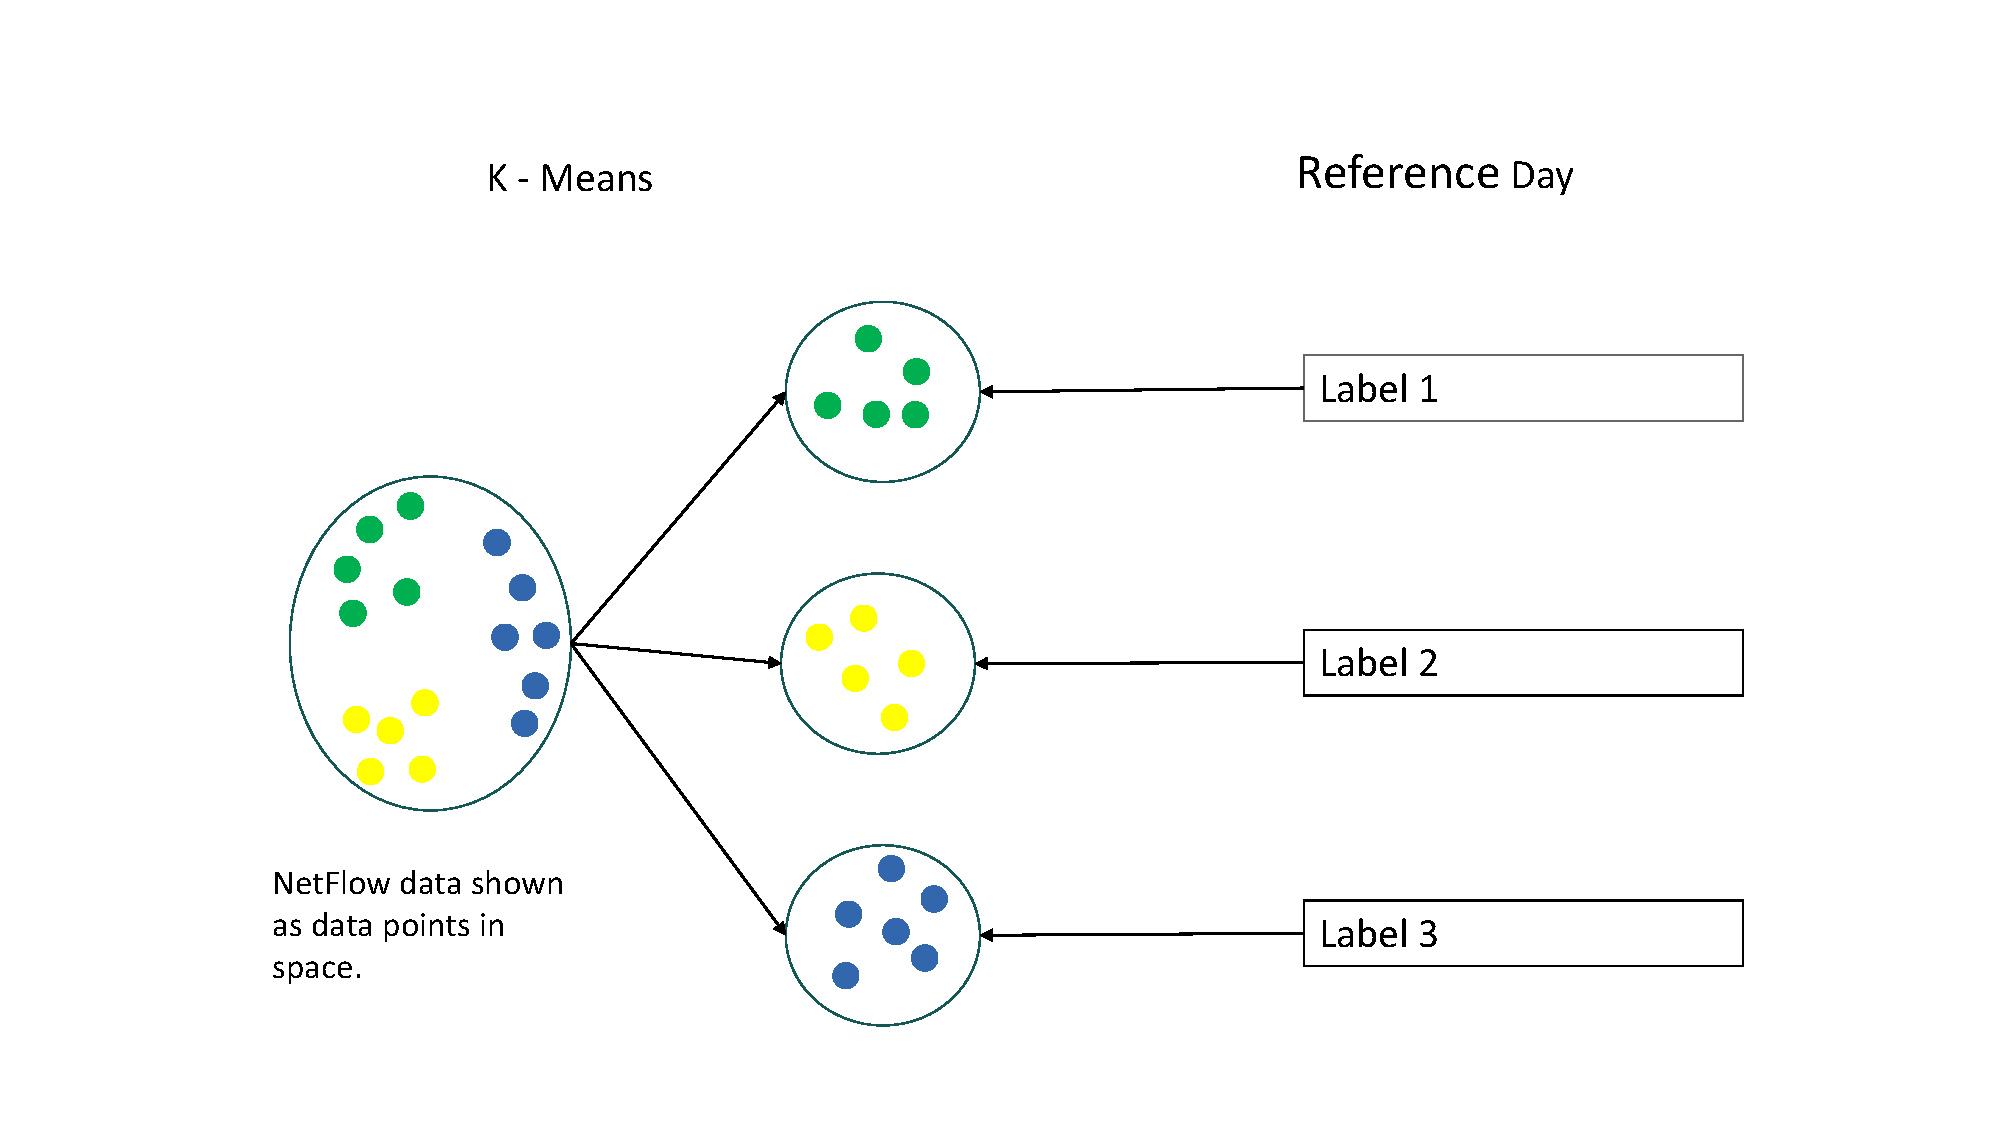
\includegraphics[scale = 0.5]{cluster_comp.pdf}}
	\caption{Process diagram on a reference day, with netflow eight dimensional data aggregated based on host shown as a 2D data point which when passed through our pattern detector split into three clusters. These clusters are manually inspected and labeled accordingly. }%
	\figlabel{cluster_comp}
\end{figure}

 Now for every other day we compare the clusters formed on that given day with the reference day. Cluster comparison is an active research area and there are very few techniques to do this and hence we solved it by converting our cluster comparison problem in to an assignment problem. An assignment problem generally deals with assigning machines to tasks, workers to jobs etc.. The goal is to determine the optimum assignment that, for example, minimizes the total cost. The assignment problem is a fundamental problem in the area of combinatorial optimization. It has many polynomial time implementations and one of them is Hungarian Algorithm \cite{}. So, in our case the assignment problem is assigning the clusters on a given day to the clusters on the reference day. We use hungarian algorithm to solve this cluster assignment. As per this algorithm a cluster on a given day gets mapped to the cluster on a reference day based on the amount of effort it takes to move all the data points from this cluster to any of the reference day clusters center. Overall the goal is to make the assignments in such a way that the total effort is least. The least effort assignment for dec 12th is shown in the \figref{assign_prob}.
 

A point to be noted here is that we might need to change the reference day with time. This could be because of change in the usage of applications over time. Our recommendation is to choose a reference day that suggests the changed behavior and keep visiting this periodically.

 \begin{figure}[b]
	\centerline{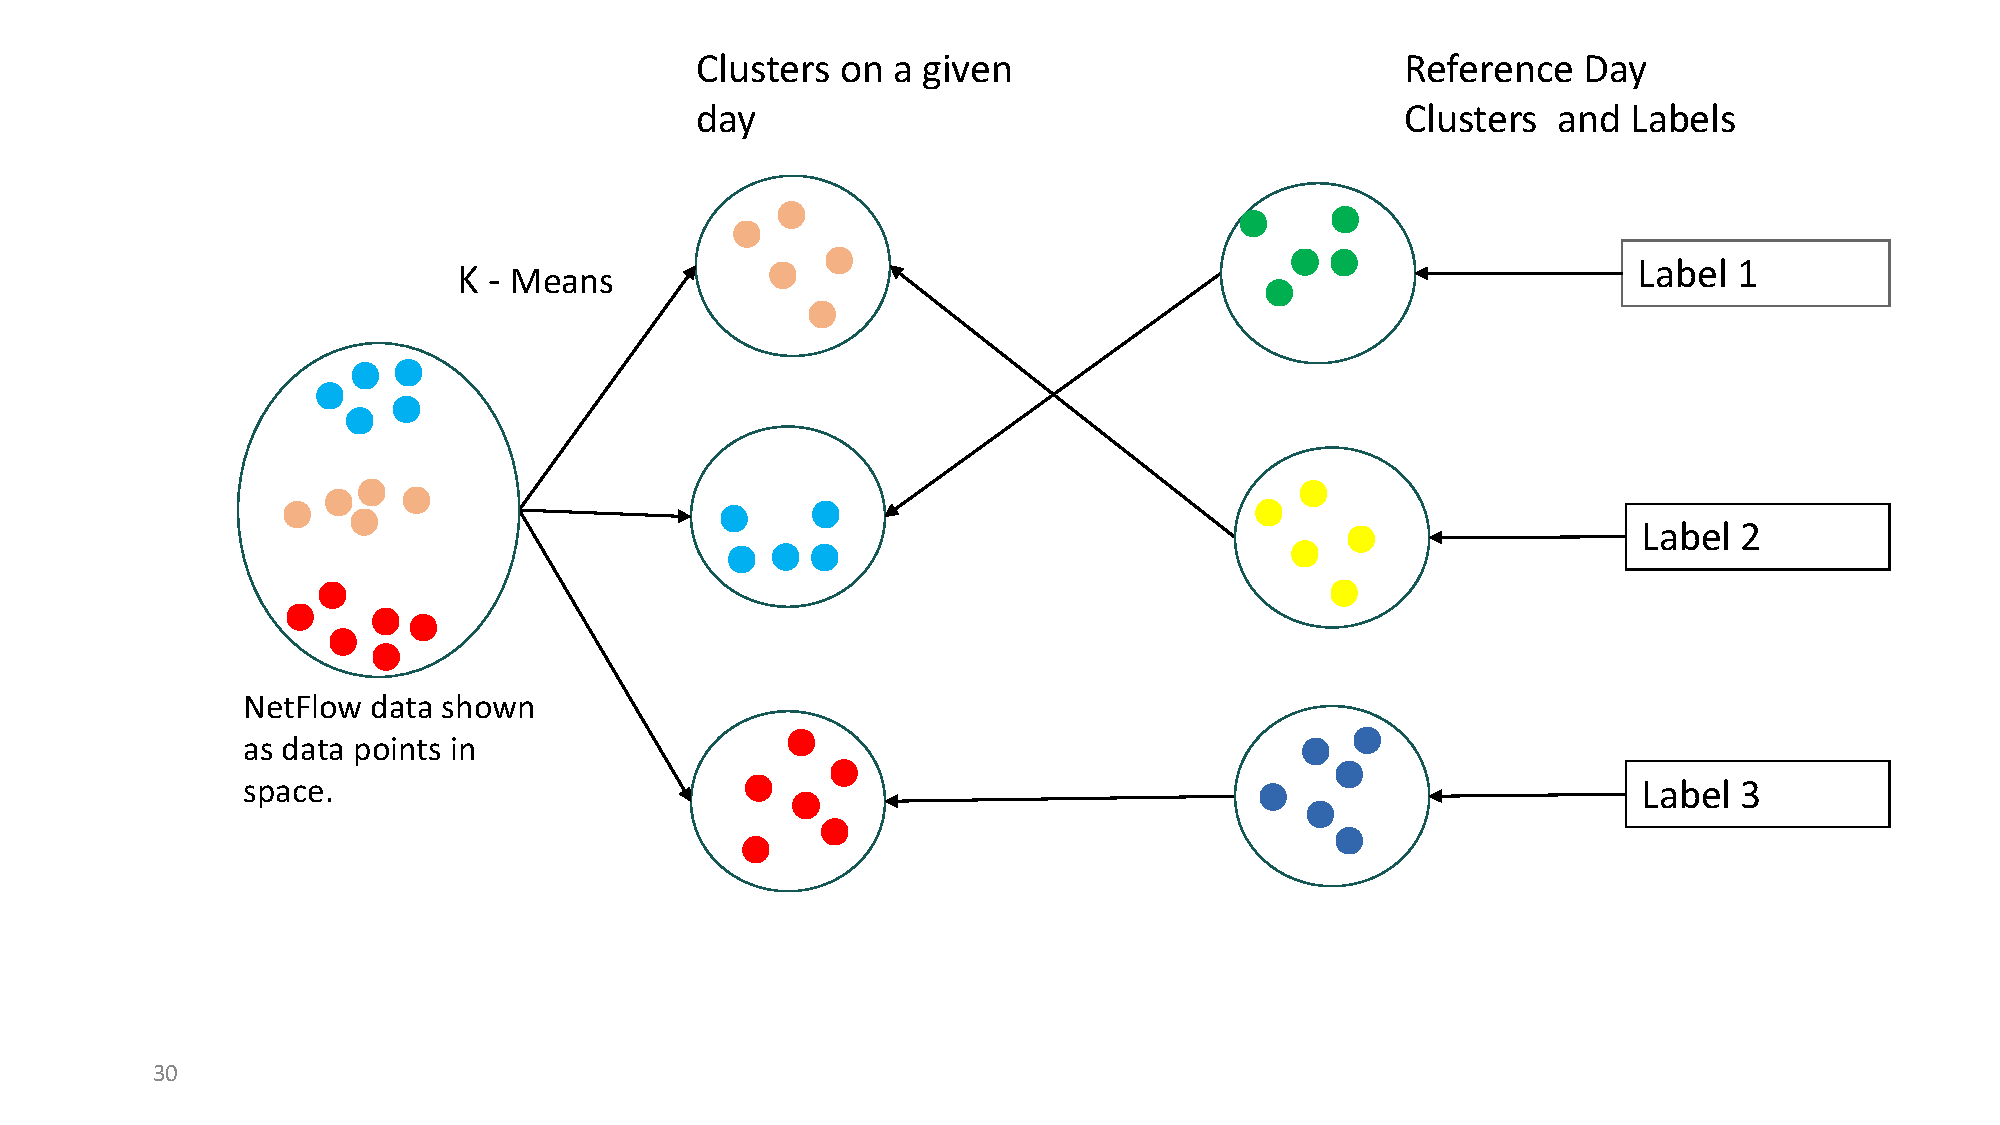
\includegraphics[scale = 0.5]{assign_prob.pdf}}
	\caption{Process diagram on a reference day, with netflow eight dimensional data aggregated based on host shown as a 2D data point which when passed through our pattern detector split into three clusters. These clusters are manually inspected and labeled accordingly. }%
	\figlabel{assign_prob}
\end{figure}
% WE can write about why we ended up with log normalization%
% Few numbers like number of code lines, programming languages used, machines on which or code is run machines on which the data is collected, data size every day, into evaluation --> execution time for each step after the nfdump we again have manual scripts to move data to other machines and from there we captre it in csv file. here these scripts are also used to feed the data into solarwinds like applications which does port based classification and we have used this technique for evaluations also.  %